\documentclass[12pt]{report}
\usepackage[margin=1in]{geometry}
\usepackage{setspace} % for single/doublespacing commands
\usepackage{graphicx} % including graphics
\usepackage{sectsty} % sexy section headings
\usepackage[export]{adjustbox} % for graphic frames and center
\usepackage{siunitx}
\usepackage{lmodern} % font package for above
\usepackage[justification=centering]{caption} % figure captions (force centering)
\usepackage{enumitem} % add arguments for enumerate to change style
\usepackage[list=true]{subcaption} % subfigures with list of figure support
\usepackage{multirow}
\usepackage{booktabs}
\usepackage{color}
\usepackage{ulem}
\usepackage[numbers]{natbib}
\usepackage{contour}
\usepackage{tabularx}
\usepackage{framed}
\usepackage{amssymb} % special math symbols
\usepackage{listings}
\usepackage{array}
\usepackage{fancyhdr}
\usepackage{color, colortbl}
\usepackage{tocloft}
\usepackage{url}
\usepackage{etoolbox}
\usepackage{hyperref}

\setlength{\parskip}{\baselineskip}%
\setlength{\parindent}{0pt}%
\setcounter{secnumdepth}{5}
\renewcommand{\bibname}{References}
\sisetup{output-exponent-marker=\ensuremath{\mathrm{e}}}
\newcommand{\PreserveBackslash}[1]{\let\temp=\\#1\let\\=\temp}
\newcolumntype{C}[1]{>{\PreserveBackslash\centering}p{#1}}
\newcolumntype{R}[1]{>{\PreserveBackslash\raggedleft}p{#1}}
\newcolumntype{L}[1]{>{\PreserveBackslash\raggedright}p{#1}}
\lstMakeShortInline[style=Matlab-editor]| % matlab inline escape character
\graphicspath{{images/}}
\renewcommand\thesection{\arabic{section}}
\renewcommand\labelitemi{---}
\lstset{numberstyle=\ttfamily\small\color{gray}}

\apptocmd{\sloppy}{\hbadness 10000\relax}{}{}
\setlength{\cftbeforetoctitleskip}{-2em}
\allsectionsfont{\raggedright}
\setlist[enumerate]{wide=0pt, widest=99,
                    leftmargin=\parindent,topsep=0pt,partopsep=0pt,
                    label=\thesubsubsection.\alph*,font=\itshape}

\begin{document}
\normalem
\begin{titlepage}
\flushleft
\doublespacing
\Large
\textsc{Test Document} \\
\normalsize
Trey Dufrene, Zack Johnson, David Orcutt, Alan Wallingford, Ryan Warner
\vfill
\center
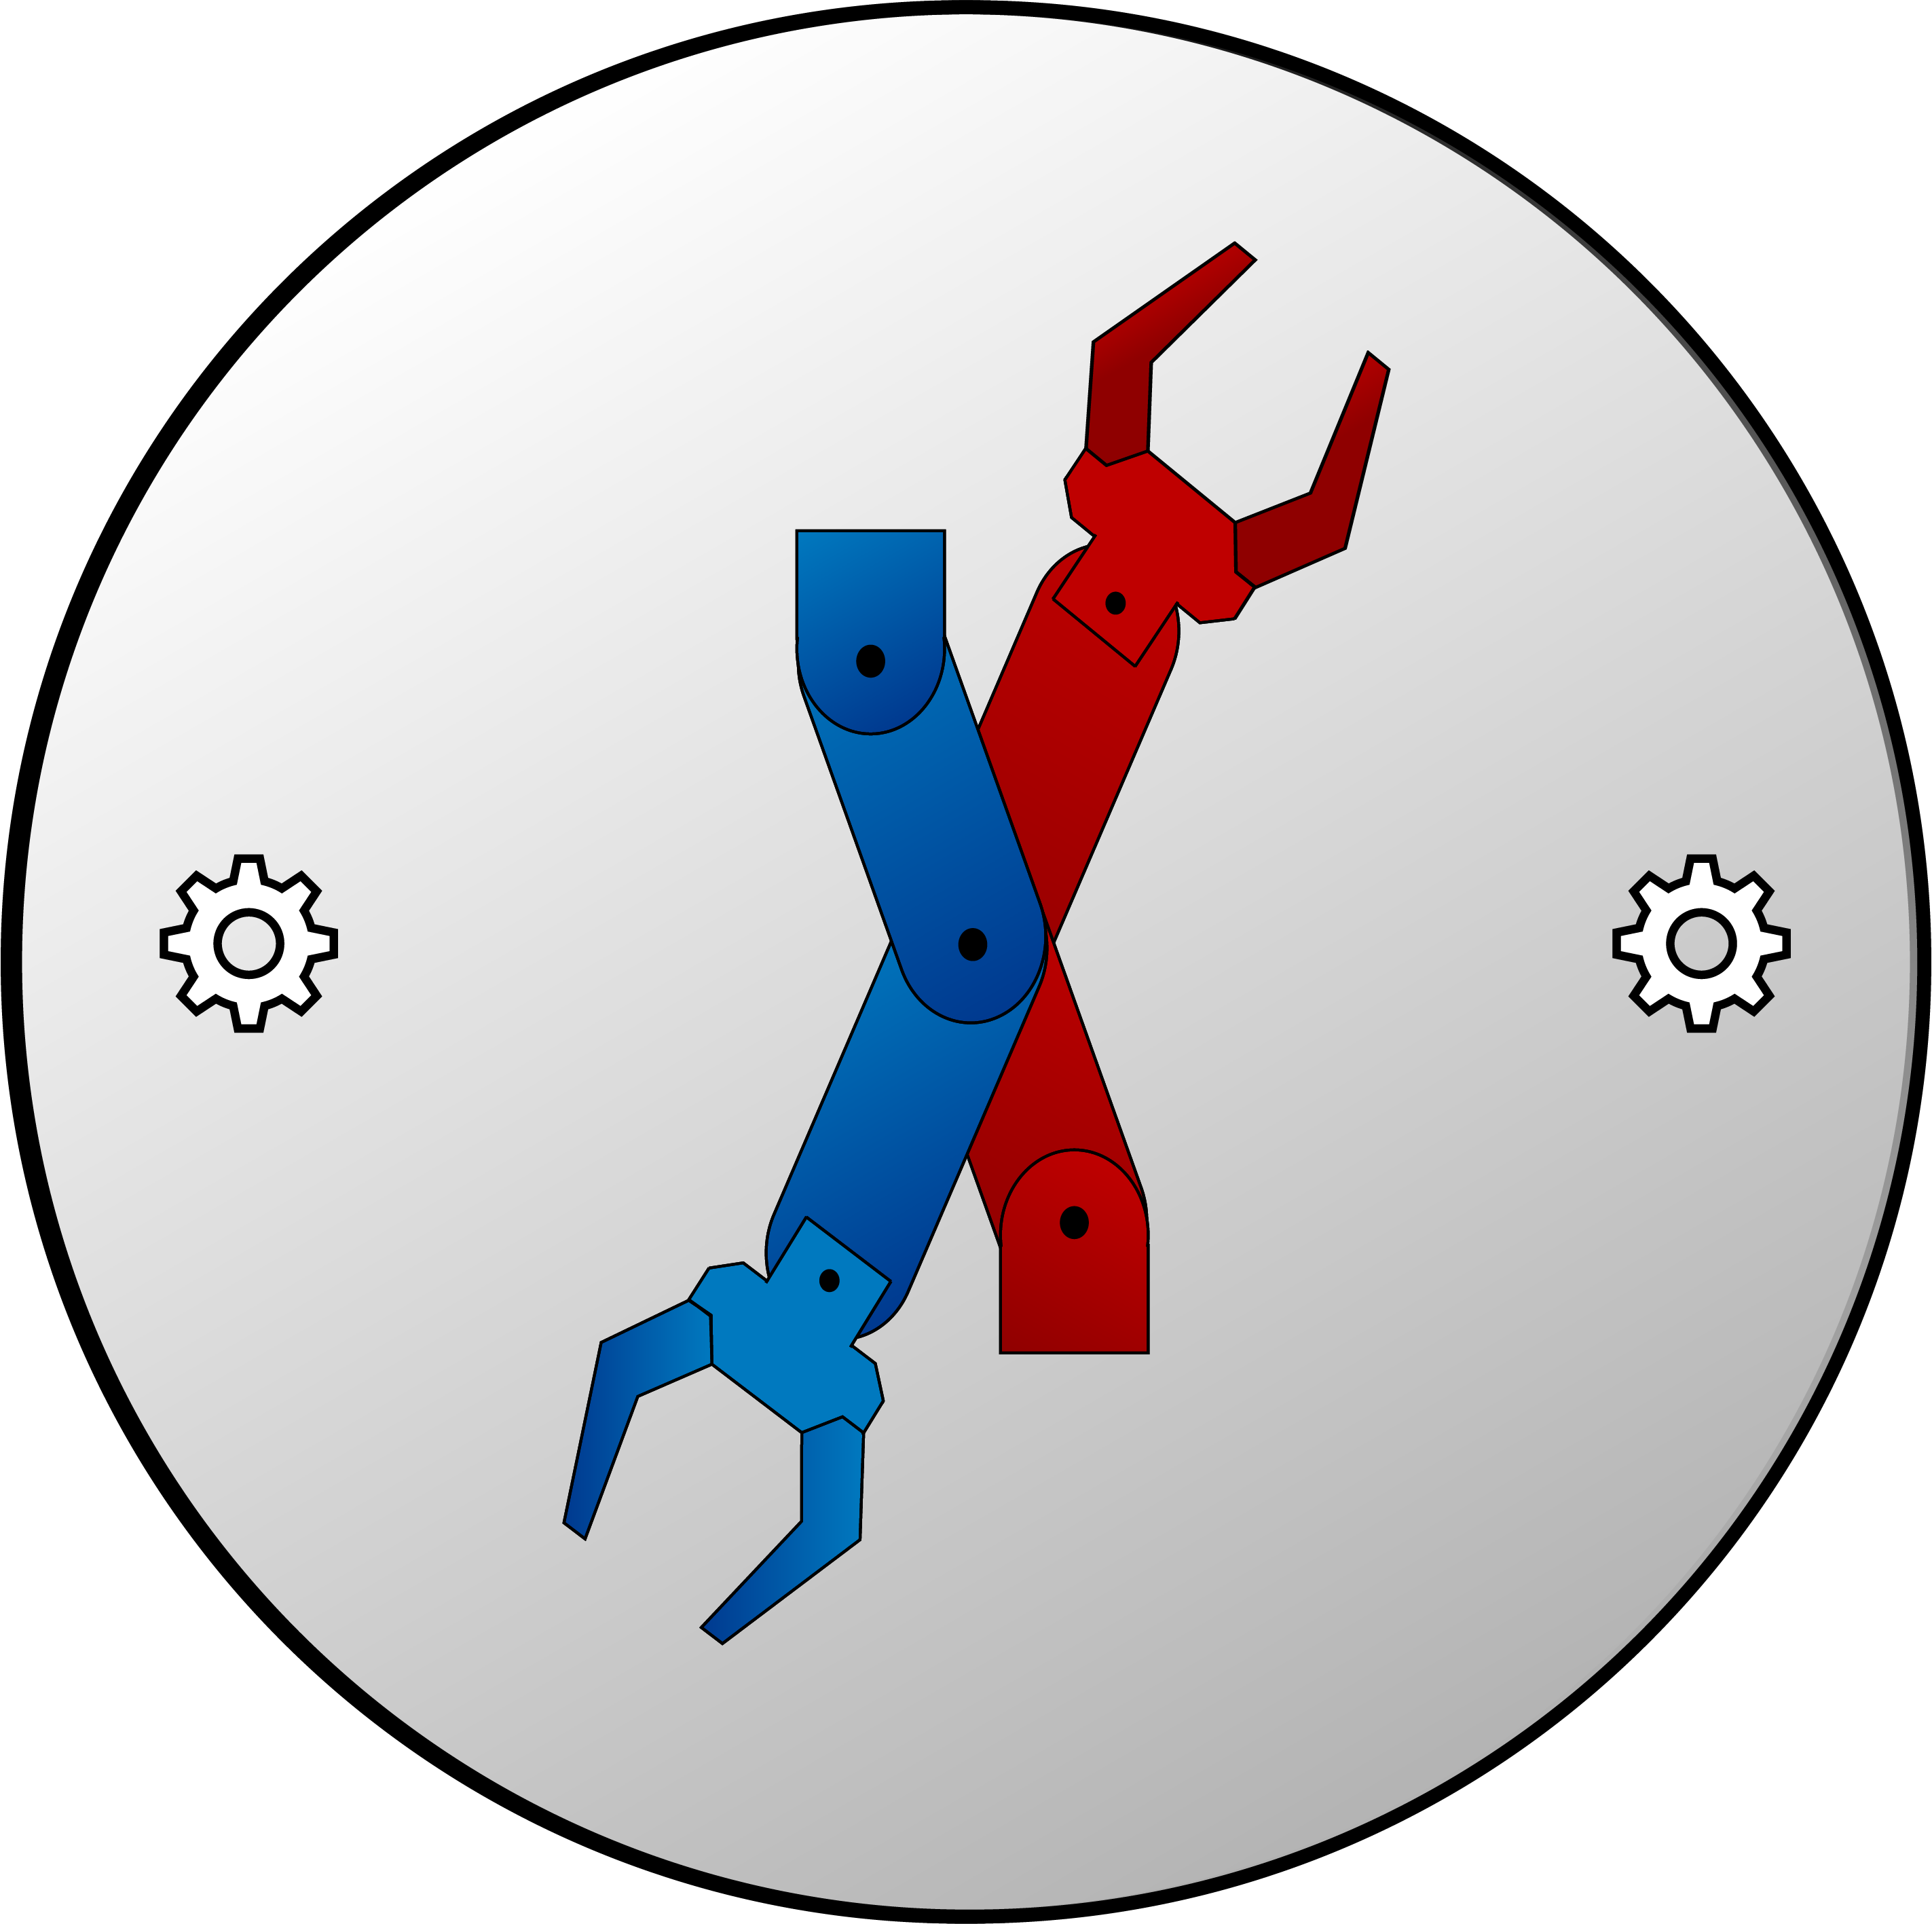
\includegraphics[width=.45\textwidth]{logo}
\vfill
\flushleft
ME 407 \\
Preliminary Design of Robotic Systems \\
Embry-Riddle Aeronautical University \\
\vspace{2ex}
\begin{minipage}[c]{.5\textwidth}
\flushleft

\includegraphics[width=.95\textwidth]{erau}
\end{minipage}%
\begin{minipage}[c]{.5\textwidth}
\flushright

\includegraphics[width=.8\textwidth]{text}
\end{minipage}
\end{titlepage}

\pagenumbering{roman}
% \begin{abstract}
  % Wordy words
% \end{abstract}
{\tableofcontents\let\clearpage\relax\listoffigures}
\clearpage
\newpage
\pagenumbering{arabic}

\section{Introduction}\label{sec:intro}
\raggedright
With the intention of making robotics education more accessible, The Manipulator for Educational Institutions with Open Source Integrated Systems (MEIOSIS) intends to provide high school educators and robot enthusiasts with a low cost manipulator. The system should be usable by novice students. It should also be modifiable to create a sustainably increased understanding of robotics. While MEIOSIS may not fully emulate industrial manipulators, it aims to provide more students with access to robotics education.
\newline\newline
The design which will be referenced throughout this document can be seen in \emph{Figure \ref{fig:model}}.
\begin{figure}[htp]
  \centering
  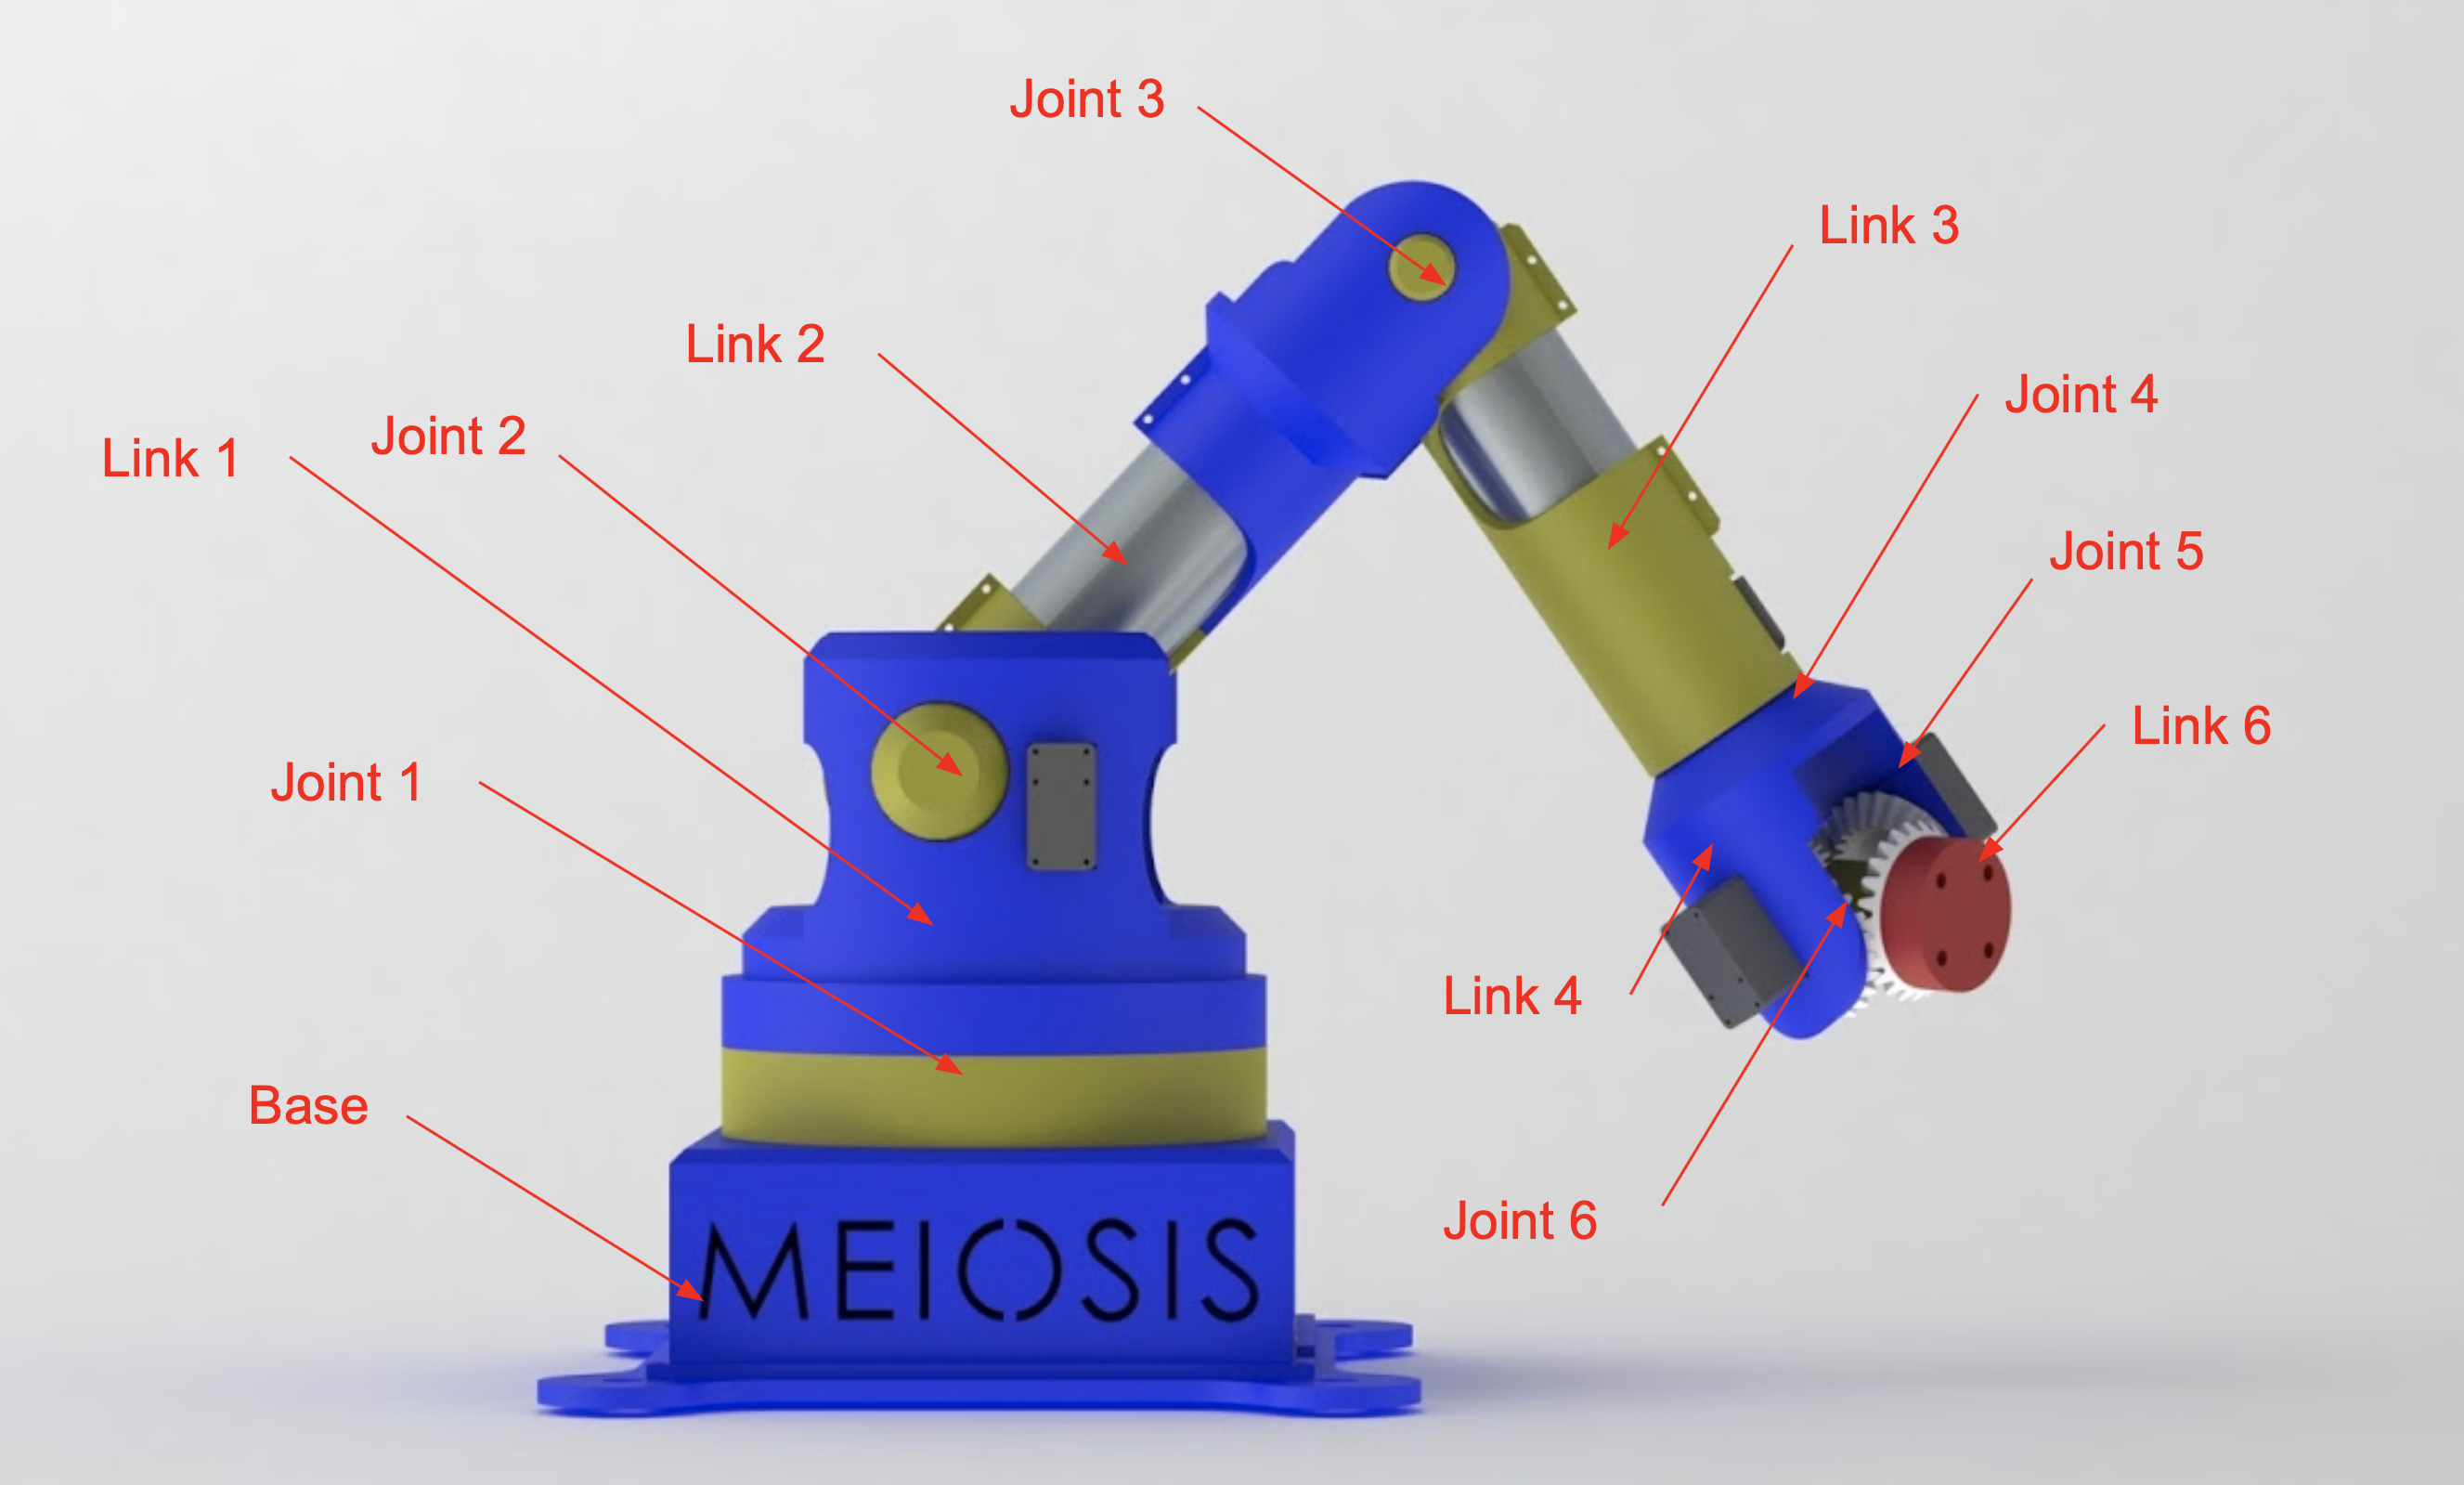
\includegraphics[frame,width=.75\textwidth]{model}
  \caption{Overview of Physical System}
  \label{fig:model}
\end{figure}
\newline
The design seen in \emph{Figure \ref{fig:model}} is based on our conceptual design. It features four links and six joints for rotation and will be referenced throughout this document. The base of the manipulator and end-effector can also be seen in the figure.
\section{Design Requirements}
The specifications of the system are strictly based on the previously defined requirements. The requirements are divided into two categories: hardware and software.
\vspace{-\baselineskip}
\subsection{Hardware}
The following requirements and specifications are hardware specific, dictating the physical system's constraints.
\vspace{-\baselineskip}
\subsubsection{The system shall cost the end-user no more than \$1000.}
\begin{enumerate}
  \item \textit{The cost for the MEIOSIS team to develop the manipulator shall be no more than \$800.}
\end{enumerate}

\subsubsection{The system shall be fully dexterous without being kinematically redundant.}
\begin{enumerate}
\item \textit{The system shall consist of six rotational joints connected by four links. The last three joints will create a spherical wrist.}
\end{enumerate}
By definition, “A manipulator having more than six DOF is referred to as a kinematically redundant manipulator [1, pp. 5].” A manipulator with less than six degrees of freedom (DOF) will not be fully dexterous within it's workspace. \emph{Figure \ref{fig:zero}} (see subsection \ref{sec:zero}, p. \pageref{fig:zero}) shows a six degree-of-freedom rotary manipulator with it's coordinate frames in zeroed positions. The joint and link locations are shown in \emph{Figure \ref{fig:model}} (see section \ref{sec:intro}, p. \pageref{sec:intro}).
\begin{enumerate}[resume]
\item \textit{The system shall have no link offsets.}
\end{enumerate}
Link offsets as seen in \emph{Figure \ref{fig:offset}} are commonly used to avoid singularities. However, having a link offset prevents the manipulator's dexterous workspace from being a complete hemispherical shell.\\
\begin{figure}[htp]
  \centering
  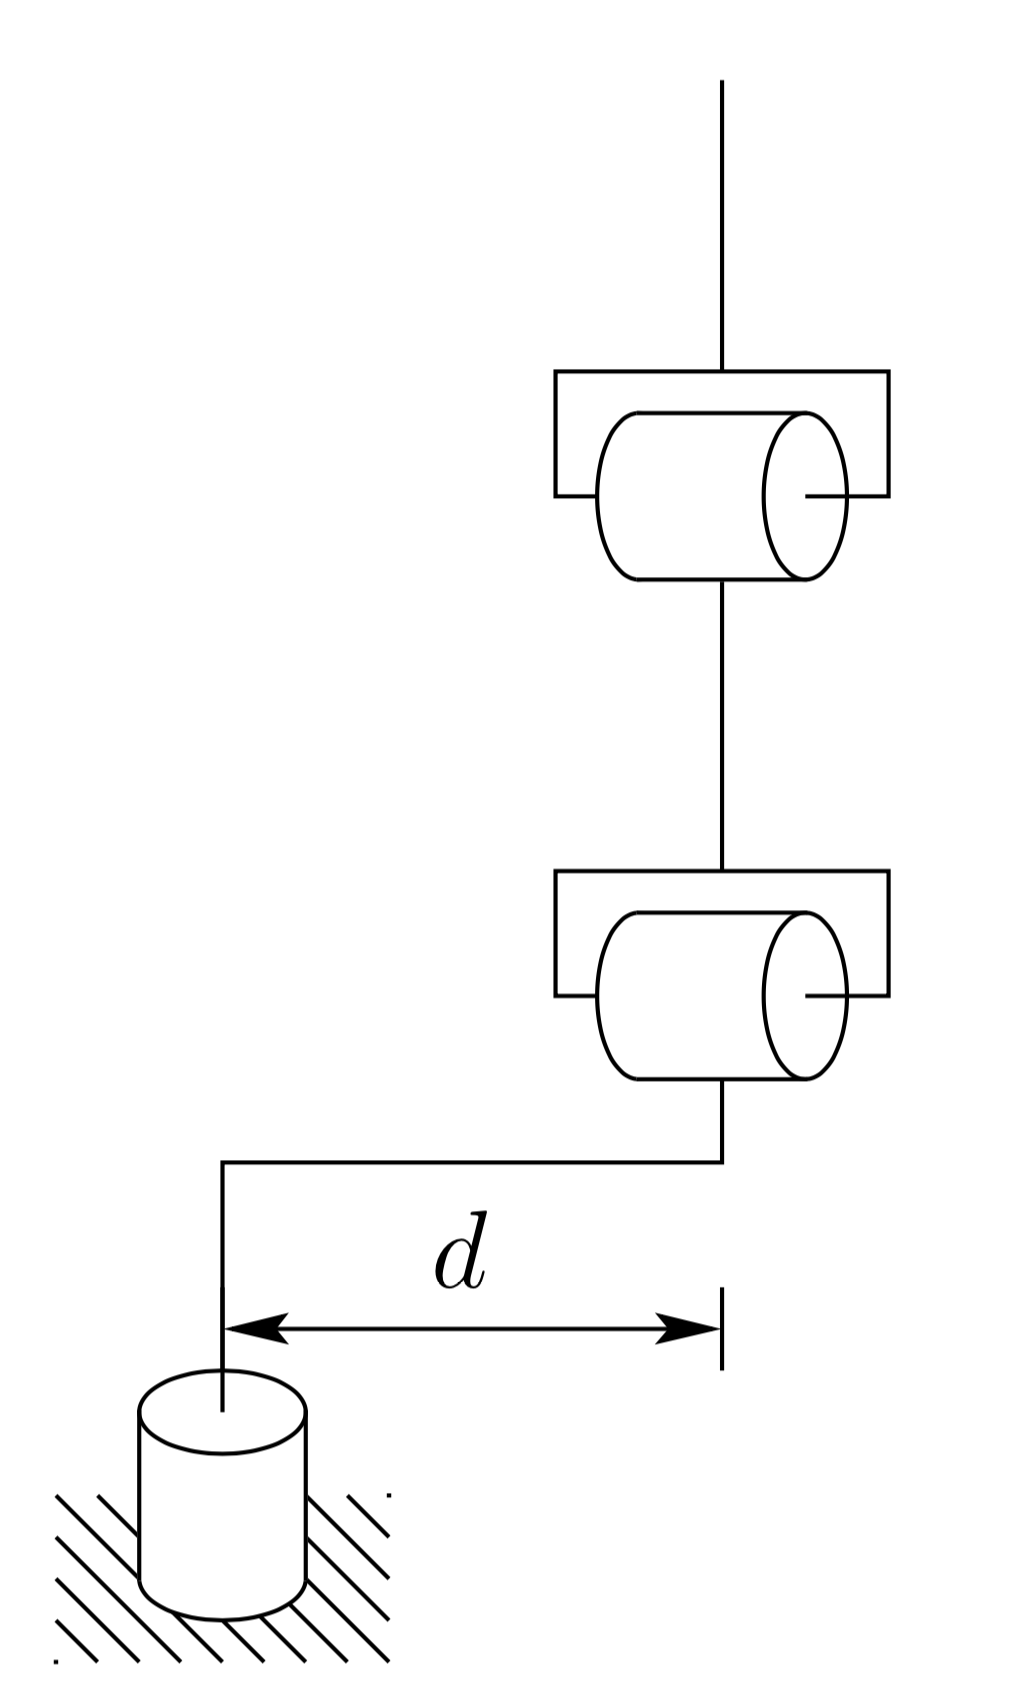
\includegraphics[width=.25\textwidth]{offset}
  \caption[Elbow Manipulator Configuration with Link Offset]{Elbow Manipulator Configuration with Link Offset \cite{robo}}
  \label{fig:offset}
\end{figure}
As shown in \emph{Figure \ref{fig:offset}}, the line directly above the first joint of the manipulator is offset such that the axes of the other joints are unable to become collinear with the base axis; this prevents singularity but causes a void in the detxterous workspace.
\subsubsection{The system end-effector shall maintain a positional accuracy magnitude of \(\pm 1\) mm and an orientation accuracy of \(\pm 5^{\circ}\) eigen angle from the base frame.}
To ensure that the robot has educational value, the accuracy must be defined so that any desired positions and movements are achieved.
\begin{enumerate}
  \item \textit{The system shall accommodate a process in which the end user can calibrate the end-effector's position and orientation to within 0.5 mm and 1 degree of the manipulator’s precision.}
\end{enumerate}
The addition of a calibration process allows the removal of any systematic errors, such as drift. The theoretical limit of the calibration process is the difference between the precision and accuracy metrics of the system.
\subsubsection{The system end-effector shall maintain a pose repeatability magnitude between 0.1—1.5 mm for the position and \(\pm 4^{\circ}\) eigen angle from the base frame for the orientation.}
\begin{enumerate}
  \item \textit{Joints one and two of the system shall possess an angular error of no more than .025 degrees.}
\end{enumerate}
Since joints one and two are the first two rotational elements in the system, their error will propagate the most to the end-effector's position.
\begin{enumerate}[resume]
  \item \textit{Joint three of the system shall possess an angle error of no more than .03 degrees.}
\end{enumerate}
Since joint three is closer to the end-effector it's error will not propagate as severely throughout the system.
\begin{enumerate}[resume]
  \item \textit{Joints four, five, and six shall possess an angle error of no more than .29 degrees.} \\
\end{enumerate}
The spherical wrist is the closest to the end-effector's final position and therefore has the least error propagation.

\subsubsection{The system’s reachable workspace shall be a hemisphere with a radius of 300-700 mm.}
This workspace will provide enough movement to manipulate objects in order to perform basic tasks.
\begin{enumerate}
  \item \textit{The length of link one, two, three, four, and the wrist shall be 220.8 mm, 250 mm, 200 mm, 80 mm, and 52.5 mm respectively.}
\end{enumerate}

\subsubsection{The system’s dexterous workspace shall contain a hemispherical shell within the reachable workspace with a thickness of 280 mm.}\label{sec:zero}
This workspace will provide enough movement to manipulate objects in order to perform basic tasks. 280mm is slightly greater than the length of letter paper.
\begin{enumerate}
  \item \textit{The rotational limit of joint one, two, three, four, five, and six shall be \(\pm180^{\circ}\), \(-9.7^{\circ}\) to \(177.5^{\circ}\), \(-150.6^{\circ}\) to \(-19.3^{\circ}\), \(\pm180^{\circ}\), \(-180^{\circ}\) to \(-1.6^{\circ}\), and \(\pm180^{\circ}\) respectively.}
\end{enumerate}
The angles stated are with respect to the kinematic model shown in \emph{Figure \ref{fig:zero}}. To be fully dexterous within the 280 mm dexterous workspace, the manipulator must have the joint angles specified above. The joint limitations were calculated by iteratively verifying the orientation about every point within the quarter hemisphere cross section seen in \emph{Figure \ref{fig:dex}} (see Appendix, p. \pageref{sec:app}).
  \begin{figure}[htp]
    \centering
    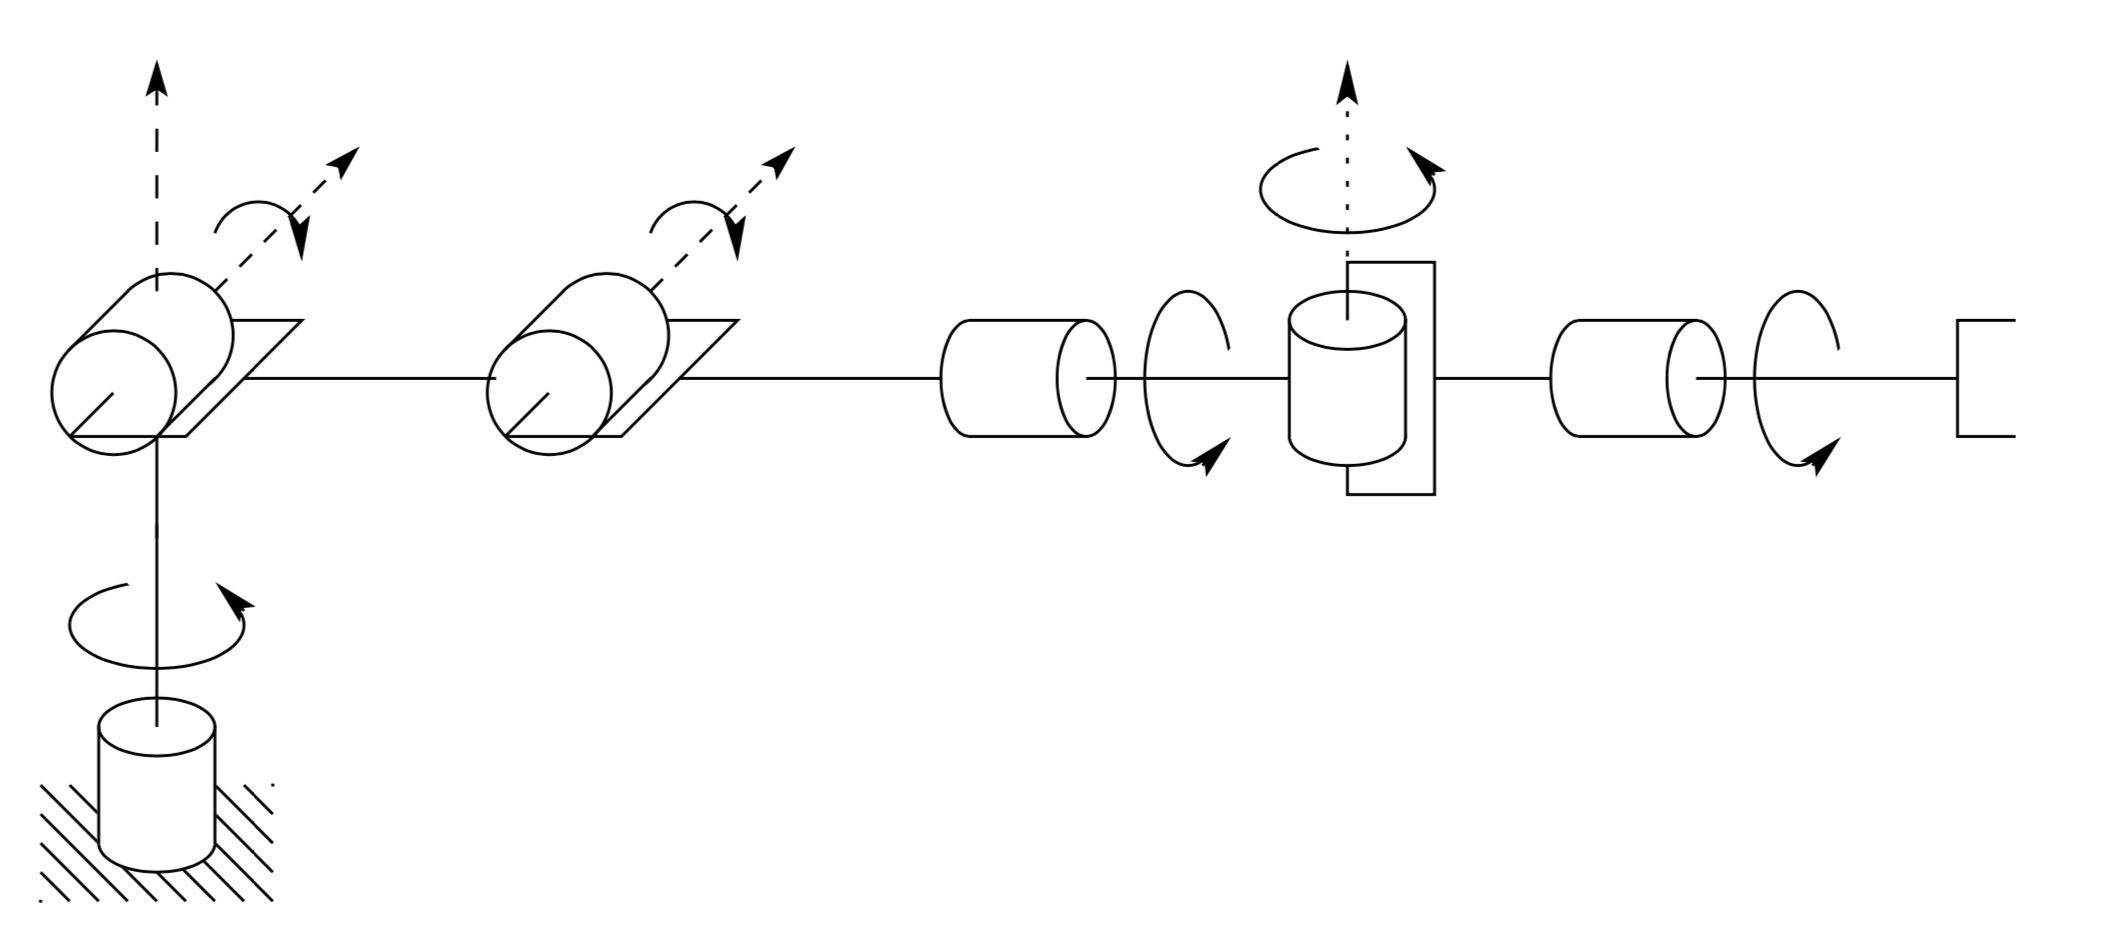
\includegraphics[width=.75\textwidth]{zero}
    \caption[Kinematic Model Representing Zeroed Configuration]{Kinematic Model Representing Zeroed Configuration \cite{robo}}
    \label{fig:zero}
  \end{figure}
\newline
The kinematic model in \emph{Figure \ref{fig:dex}} shows the zeroed configuration for a six degree of freedom robot with only rotational joints. This is the reference configuration for specifications 2.1.2.a, 2.1.5.a, and 2.1.6a.
\subsubsection{The system shall have a removable end-effector capable of picking and placing a low-odor chisel tip Expo dry erase marker.}
A removable end-effector creates a robot capable of performing a variety of basic tasks, which enhances its educational value.
\begin{enumerate}
  \item \textit{The system shall use a gripper that can close to 18mm.}
\end{enumerate}
The diameter of a low-odor chisel tip Expo dry erase marker is approximately 18 mm.
\begin{enumerate}[resume]
  \item \textit{The end-effector shall attach to the manipulator using screws configured in a pattern that can accommodate a Dynamixel AX-12A servo.}
\end{enumerate}
It is expected a majority of end-effectors will be actuated by a servo, therefore a specific servo's mounting pattern was chosen to standardize the mounting.


\subsubsection{The system shall be able to write with a low-odor chisel tip Expo dry erase marker.}
\begin{enumerate}
  \item \textit{The end-effector shall be able to support 0.004 Newton meter moments about the axes normal to its gripping surfaces.}
\end{enumerate}
  The coefficient of friction between the Expo marker and paper can be approximated and given the weight of an Expo marker the approximate moments acting on the end-effector can be calculated.
\subsection{Software}
The following requirements and specifications are software specific and determine the attributes of the operating system.
\subsubsection{The system shall be open source.}
Open source software creates an easily obtainable, low cost method of distributing the system’s source code, which may be modified for personal use.
\begin{enumerate}
  \item \textit{The software shall be hosted publicly on an online repository and maintain an MIT license for distribution.}
\end{enumerate}
  An MIT license allows the end-user to freely download and modify the code without licensing. The MIT does not legally obligate the original author maintain the code and documentation.

\subsubsection{The system shall be capable of operating given only desired end-effector cartesian coordinates specified with respect to the base frame.}
\begin{enumerate}
  \item \textit{The system shall have a user interface capable of accepting the end-effector’s desired cartesian position and Euler angle orientation as a six element row vector.}
\end{enumerate}
  The system software interface allows an untrained user to operate the manipulator without advanced knowledge of the system's kinematics.
\begin{enumerate}[resume]
  \item \textit{The system shall be capable of performing floating point arithmetic.}
\end{enumerate}
The solution for the inverse kinematics requires high level arithmetic to be preformed with little error.
\newpage
\appendix
\renewcommand\thesection{\Roman{section}}
\renewcommand\thesubsection{\roman{subsection}}
\section*{Appendix}\label{sec:app}
\begin{figure}[htp]
  \centering
  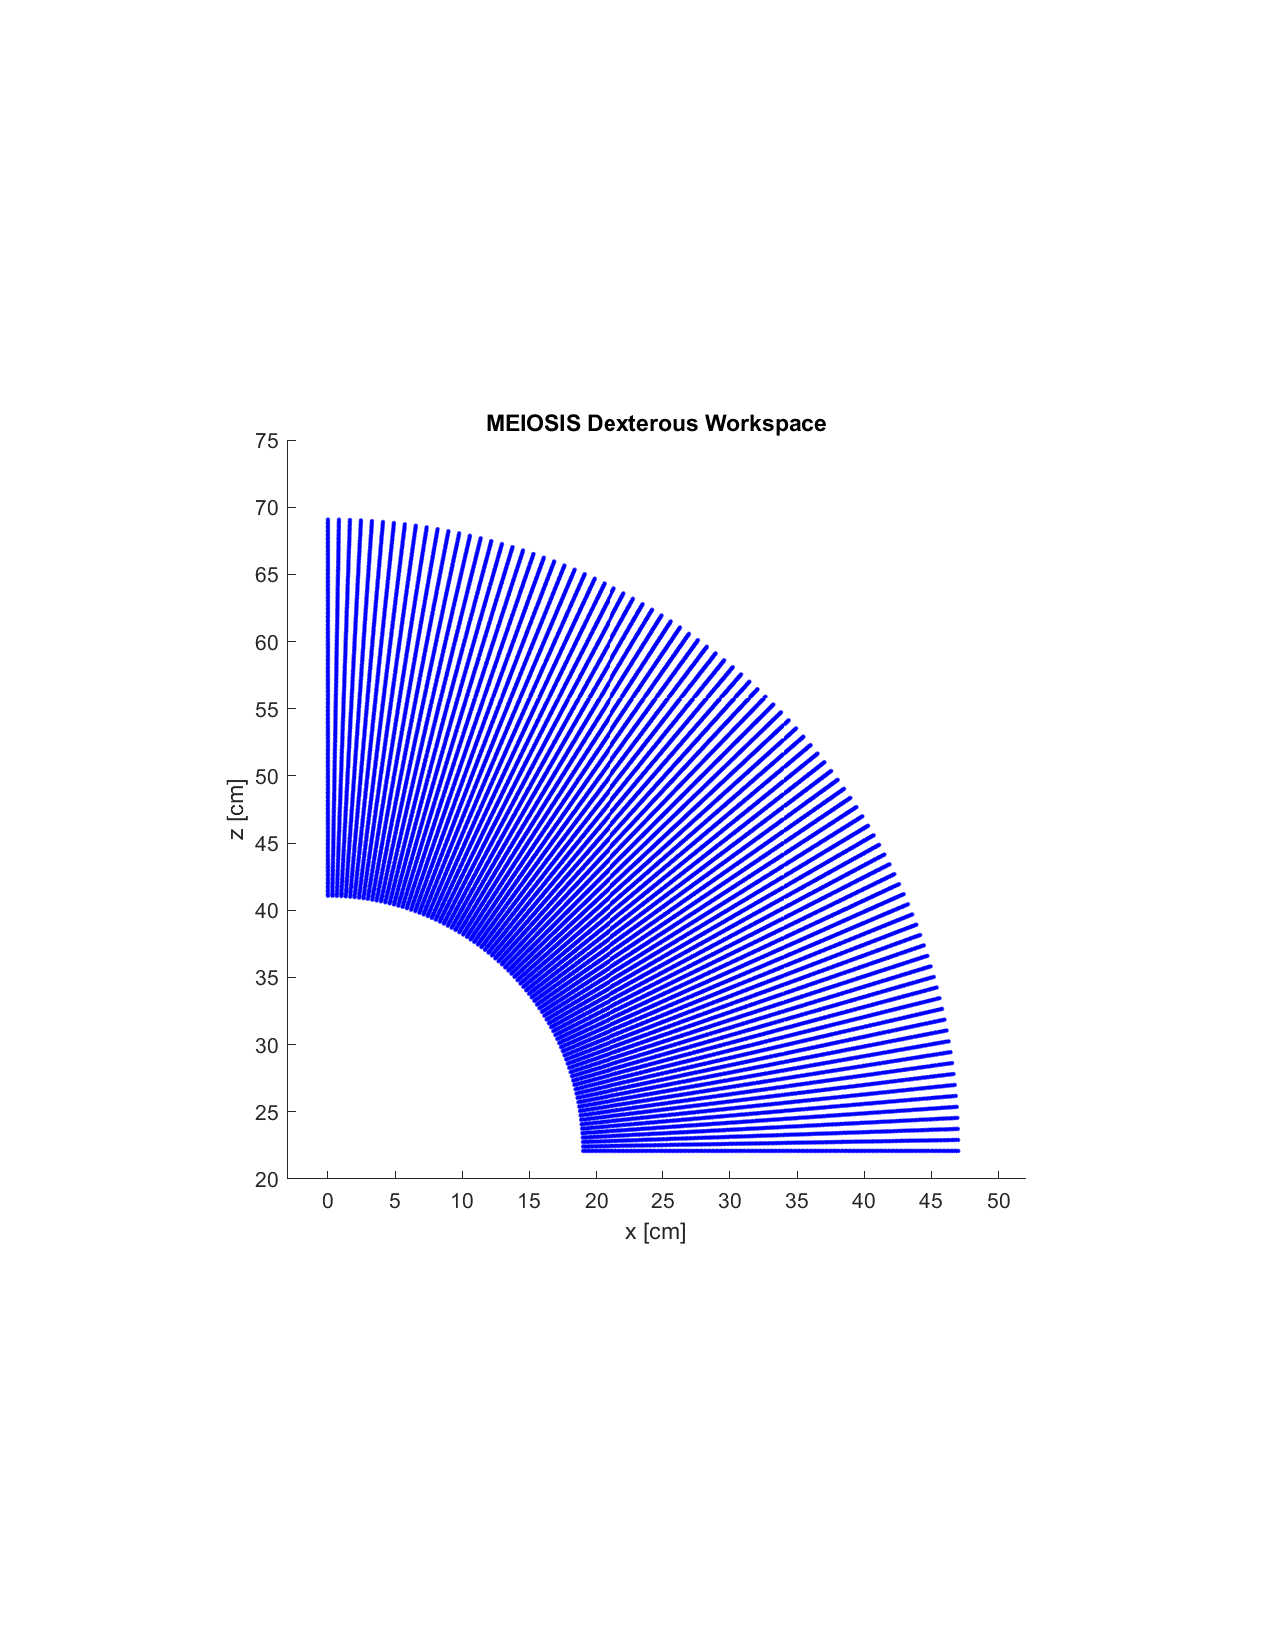
\includegraphics[frame,width=.75\textwidth]{dex}
  \caption{Cross Section of Dexterous Workspace Quadrant}
  \label{fig:dex}
\end{figure}
The plot shown in \emph{Figure \ref{fig:dex}} exhibits a cross-section of the dexterous workspace defined by requirement 2.1.6 and shows how specification 2.1.6.a was calculated. The MATLAB script that created this plot was made to show red points where the robot is not fully dexterous and the lack of red dots shows that the robot is fully dexterous within the calculated area. This also drives specification 2.1.2.b as the workspace would have red points with a link offset.

\newpage
\bibliographystyle{plainnat}
\bibliography{robo}


\end{document}
